\section{Diseño del sistema}\label{sec:diseno_del_sistema}

En la figura~\ref{fig:chapter_1.overview} vimos un esquema general del sistema, el cual recibe documentos en formato
\textit{PDF} y genera objetos que contienen la información más importante de los mismos.
Dependiendo del tipo de documento, la información contenida en estos objetos puede variar.

En la figura~\ref{fig:chapter_1.specific_b} vimos que se va a incluir también el desarrollo de dos interfaces, una
web y una de línea de comandos.

\begin{figure}[ht]
    \begin{center}
        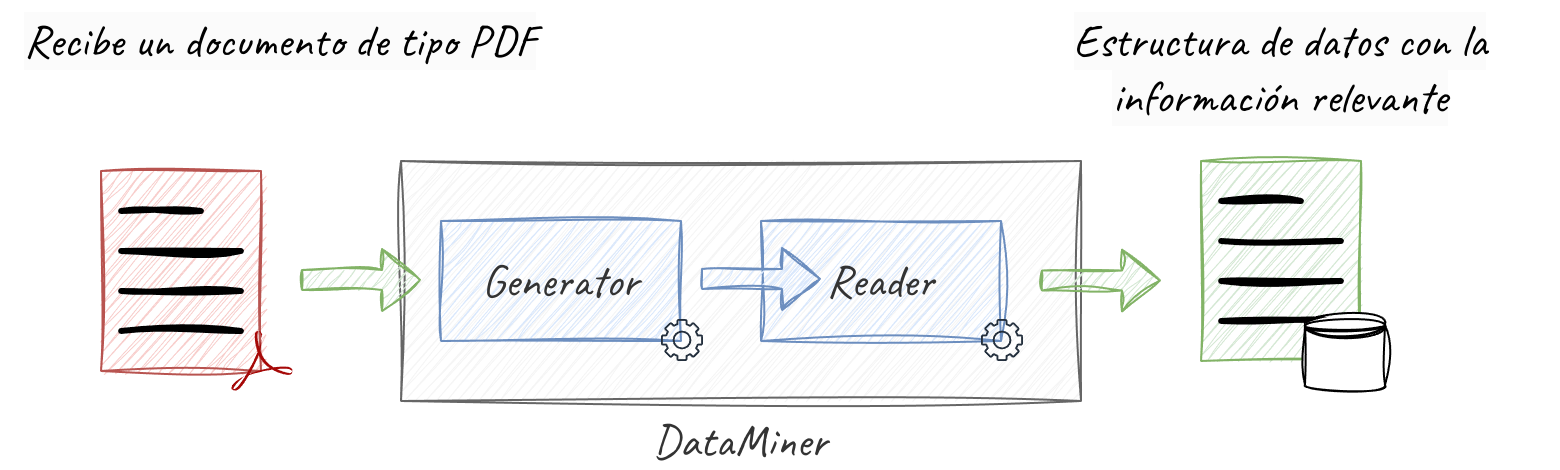
\includegraphics[width=\textwidth]{./chapter/4/images/chapter_4.1.overview}
        \caption{Esquema de los componentes principales del sistema}
        \label{fig:chapter_4.1.overview}
    \end{center}
\end{figure}

En esta sección profundizaremos en el diseño de la arquitectura de este sistema.
En la figura~\ref{fig:chapter_4.1.overview} vemos que el sistema tiene dos componentes principales: el componente
\textit{Generator} y el componente \textit{Reader}.
El primero será responsable de convertir los documentos en formato texto y el segundo de extraer la información.

\subsection*{Componente \textit{Generator}}\label{subsec:chapter_4.generator_component}

La responsabilidad de este primer componente, el \textit{Generator} es convertir archivos de cualquier formato en una
representación en texto plano del mismo.
Tal y como se ve en la figura~\ref{fig:chapter_4.1.generator_component_uml} con el esquema \textit{UML} el componente
consta de cuatro tipos diferentes de elementos.

\begin{figure}[ht]
    \begin{center}
        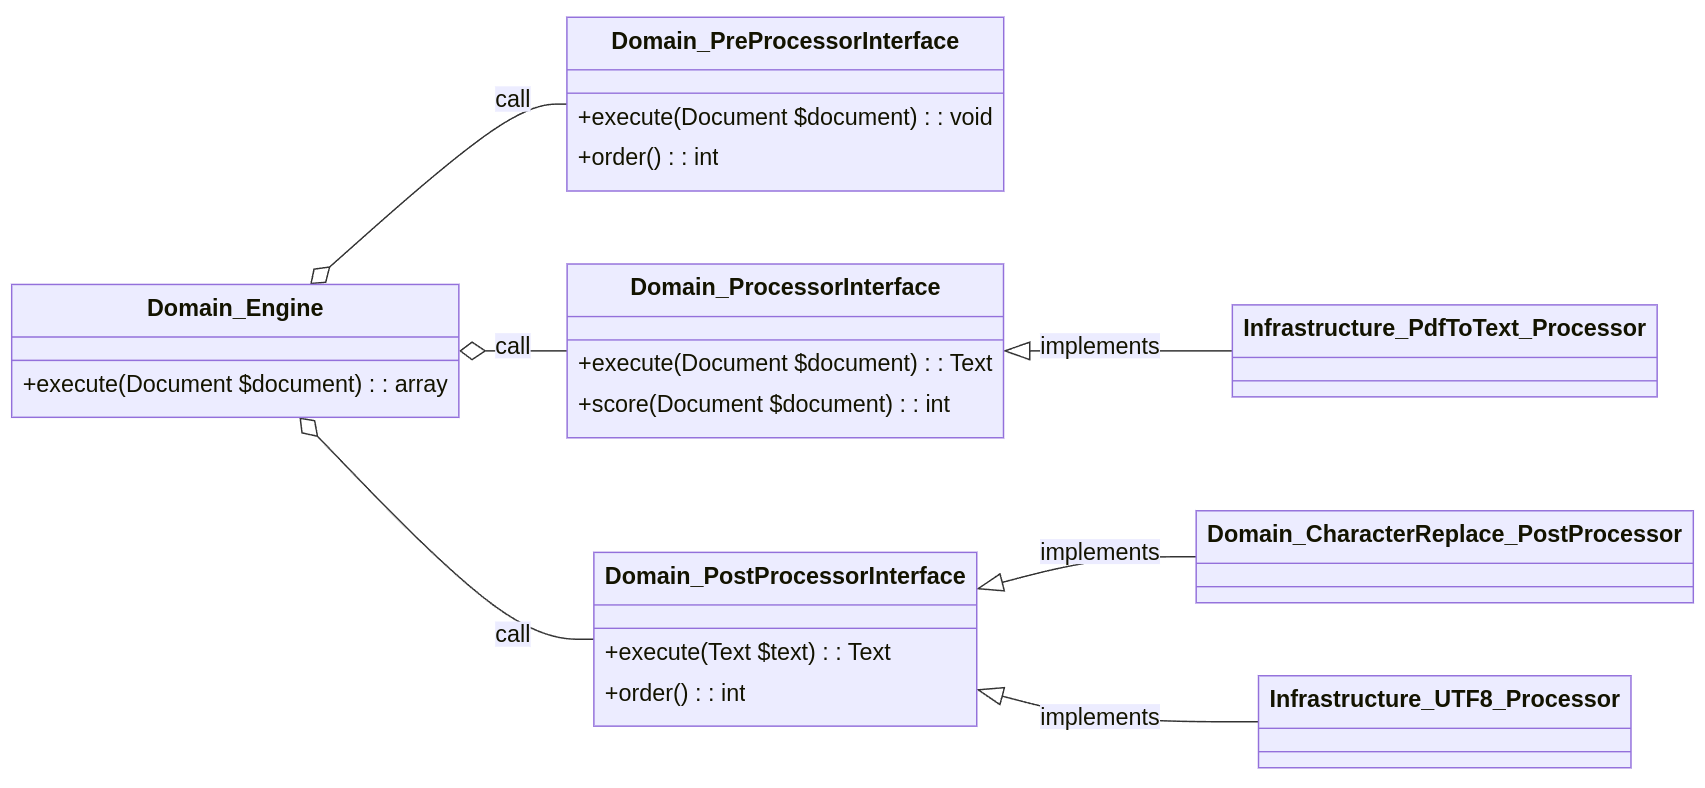
\includegraphics[width=\textwidth]{./chapter/4/images/chapter_4.1.generator_component_uml}
        \caption{Diagrama UML del componente \textit{Generator}}
        \label{fig:chapter_4.1.generator_component_uml}
    \end{center}
\end{figure}

Es importante destacar que salvo el \textit{Engine}, el resto de elementos son intercambiables, y dependiendo del caso
de uso, pueden utilizarse los componentes descritos en este TFG, o ser necesaria la implementación de otros nuevos.

El motor o \textit{Engine} es el corazón del componente.
Es el encargado de realizar las llamadas a los demás elementos registrados en el mismo coordinando cuáles y en que
orden deben ser llamados.

Los \textit{pre procesadores} preparan el documento original para facilitar su conversión a texto.
En esta implementación no se ha desarrollado ningún preprocesador, ya que no ha sido necesario para los casos de uso
previstos.

Los \textit{procesadores} realizan la conversión efectiva del documento a texto.
Funcionan mediante un sistema competitivo donde varios procesadores evalúan su propia aptitud para manejar el
formato del en cuestión, seleccionando cuál es el más adecuado para llevar a cabo la tarea.

En la figura~\ref{fig:chapter_4.1.generator_component_processors} puede verse un ejemplo.
El \textit{Engine} pretende convertir un fichero \textit{PDF} en texto y tiene registrados dos
hipotéticos procesadores: el\textit{MP3 Processor} y el \textit{PDF Processor}.

Primero realiza una llamada a \textit{MP3 Processor}, el cual evalúa el documento y responde con una puntuación
de -1, lo cual indica que no es capaz de procesar este tipo de documento.

A continuación realiza una segunda llamada a \textit{PDF Processor}, el cual evalúa el documento y responde con una
puntuación de 90, lo cual significa que es un procesador adecuado para procesar este formato de documento.

\begin{figure}[ht]
    \begin{center}
        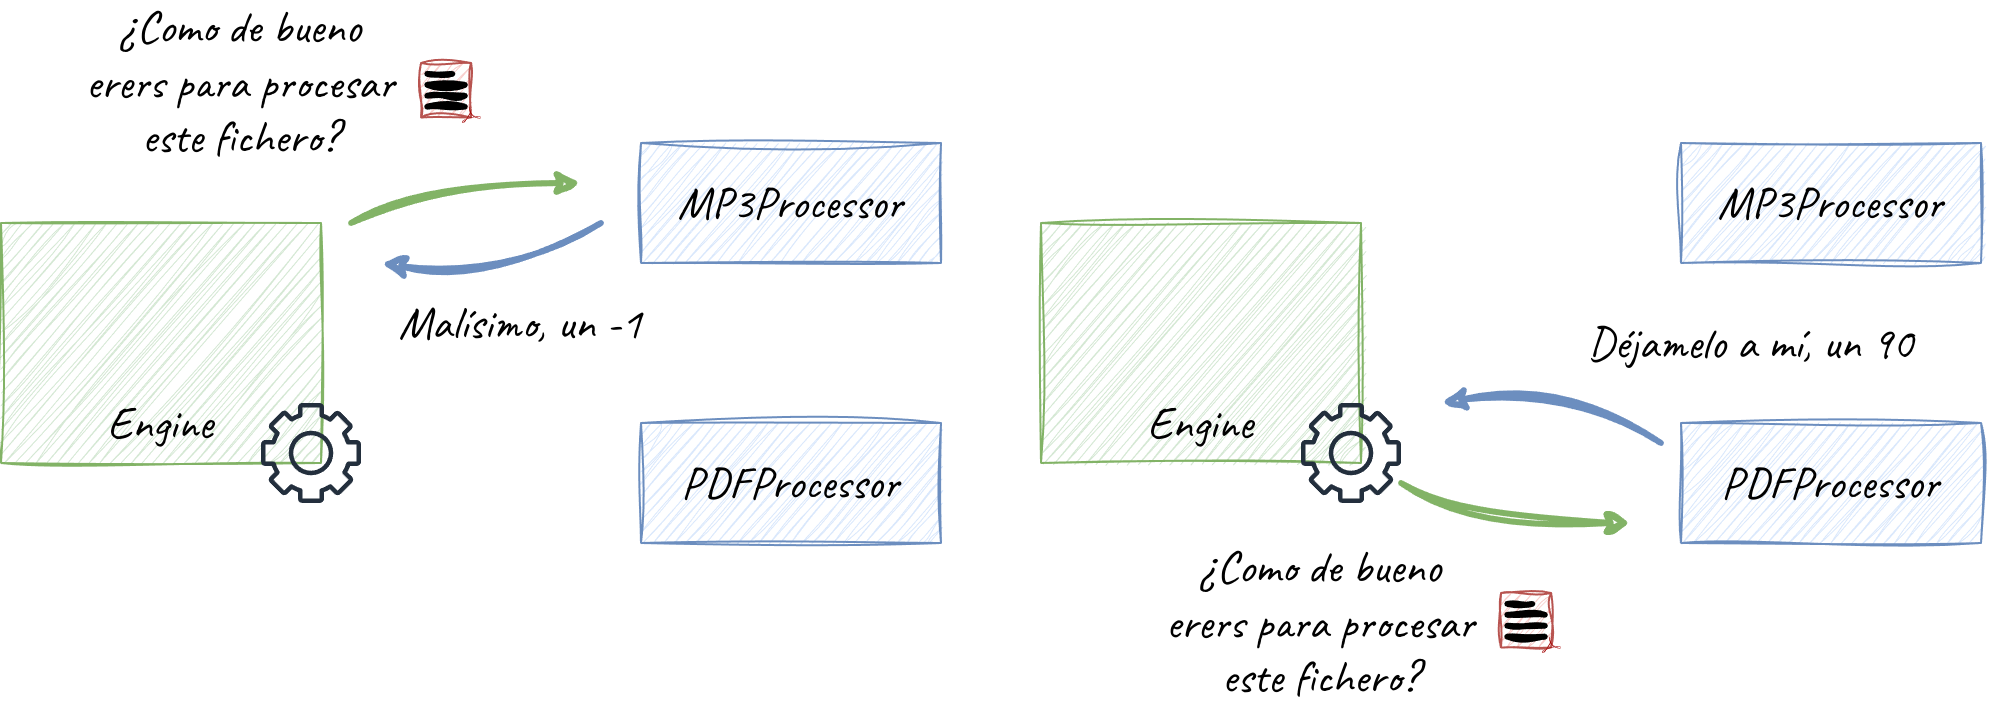
\includegraphics[width=\textwidth]{./chapter/4/images/chapter_4.1.generator_component_processors}
        \caption{Esquema de la competición entre procesadores del componente \textit{Generator}}
        \label{fig:chapter_4.1.generator_component_processors}
    \end{center}
\end{figure}

Si existieran más procesadores registrados, se irían invocando secuencialmente, para que evaluaran como de adecuados
son para procesar ese tipo de documento.
Finalmente, una vez que todos los procesadores han sido invocados, el \textit{Engine} enviará el documento al procesador
que haya respondido con una puntuación más alta.

Como puede verse, es fácil añadir soporte a nuevos tipos de documentos.
Se podría añadir soporte para documentos escaneados simplemente añadiendo un procesador que utilize una tecnología
de reconocimiento de caracteres u \textit{Optical character recognition} (OCR) como por ejemplo \textit{Tesseract OCR}
~\cite{url_tesseract}.

El \textbf{Requisito 1} definido en la sección~\ref{sec:objetives} Objetivos para este proyecto era
``convertir documentos \textit{PDF} en documentos de texto''.

El procesador \textit{PDF To Text Processor} es el responsable de esta tarea mediante llamadas a una tecnología que se
encuentra en la capa de infraestructura, en este caso \textit{Pdf to Text}~\cite{url_pdftotextl}.
Añadiremos más detalles sobre como fue la implementación de este procesador en la
sección~\ref{sec:implemetacion_y_programacion} Implementación y programación.


Los \textbf{post procesadores} perfeccionan el texto generado, realizando los ajustes necesarios, lo que mejora la
calidad del texto resultante.

Los post procesadores se llaman secuencialmente.
El primer post procesador recibe como entrada la salida del procesador ejecutado.
Los siguientes post procesadores reciben como entrada la salida del post procesador anterior.

En esta implementación, se han desarrollado los siguientes post procesadores:

\begin{itemize}
    \item
    \textbf{UTF8 Post Processor}: Ya que algunos documentos pueden contener caracteres no \textit{UTF8} este procesador
    los reemplazará por caracteres equivalentes en UTF8.

    \item
    \textbf{Character Replace Post Processor}: Después de eliminar los caracteres no \textit{UTF8} se detectó que
    algunos caracteres todavía podrían resultar problemáticos, así que se implementó un nuevo procesador capaz de
    reemplazar caracteres problemáticos, por otros equivalentes.
    En este caso se intercambió el carácter salto de página \textit{\textbackslash f}, por el carácter
    salto de línea \textit{\textbackslash n}.

    \item
    \textbf{Word Limit Post Processor}: Más adelante en la implementación del componente \textit{Reader}, y debido
    al uso de las tecnologías implementadas en el mismo, se vio que documentos con textos demasiado largos podrían
    generar errores.
    Es por esto que se decidió implementar este procesador que corta el texto después de las primeras N palabras.
\end{itemize}

En conjunto al ejecutarse los tres, primero se sustituyen los caracteres no \textit{UTF8}, por otros equivalentes, a
continuación se sustituye el carácter salto de página.
Finalmente, se determinó, para el conjunto de datos de prueba que la información relevante se encuentra siempre
dentro de las primeras dos páginas, y que en promedio cada página contenía unas 400 palabras, por motivos de
rendimiento y coste se limitó el tamaño del texto resultante a 1000 palabras.

\subsection*{Componente \textit{Reader}}\label{subsec:chapter_4.reader_component}
El componente Reader es el responsable de interpretar y procesar el texto plano obtenido a partir de la salida del
componente \textit{Generator} descrito en la subsección anterior.

Tal y como se ve en la figura~\ref{fig:chapter_4.1.reader_component_uml} el componente consta de dos tipos diferentes de
elementos: El motor o \textit{Engine} es el corazón del componente.
Es el encargado de hacer las llamadas a los demás elementos registrados en la aplicación, en este caso únicamente los
procesadores.

\begin{figure}[ht]
    \begin{center}
        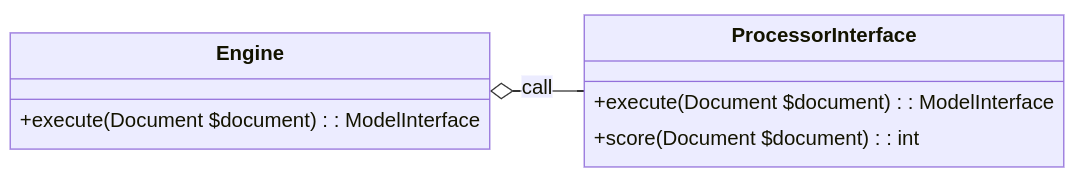
\includegraphics[width=\textwidth]{./chapter/4/images/chapter_4.1.reader_component_uml}
        \caption{Diagrama UML del componente \textit{Reader}}
        \label{fig:chapter_4.1.reader_component_uml}
    \end{center}
\end{figure}

Los procesadores están organizados en una única capa y operan bajo el mismo mecanismo competitivo descrito en la
subsección \ref{subsec:chapter_4.generator_component} Componente \textit{Generator}.

Cada uno de estos procesadores es invocado secuencialmente para evaluar su idoneidad en el manejo de un tipo de
documento específico.

Una vez seleccionado, el procesador elegido procede a ejecutar una serie de tareas que incluyen la identificación y
extracción de la información clave.

En esta implementación, se han desarrollado los siguientes procesadores:

\begin{itemize}
    \item \textbf{Residential Lease Agreement Processor} adecuado para evaluar contratos de arrendamiento de
    vivienda entre particulares tal y como indicamos en \textbf{Requisito 2}.

    \item \textbf{Vehicle Sale And Purchase Agreement Processor} adecuado para evaluar contratos de compra venta de
    vehículo entre particulares tal y como indicamos en \textbf{Requisito 3}.
\end{itemize}
